\documentclass[plainarticle,zihtitle,german,final,hyperref,utf8]{zihpub}
\usepackage{setspace}
\usepackage{listings}
\author{Bengt Lennicke}
\title{Komplexpraktikum "Paralleles Rechnen" \newline A - Stringmanipulationen mit Intrinsics}




\begin{document}

\section{Aufgabenstellung}

Implementieren Sie eine sequentielle und eine SIMD-parallele (mittels Intrinsics für einen Prozessor, der AVX2, AVX und FMA unterstützt) Variante für folgende String-Funktionen:
\begin{verbatim}
/* turns string "string" (with length len_string) to uppercase */
/* returns 1 if there has been an error, 0 if there has been no error */
int toUppercase(char* string, int len_string)

/* turns string "string" (with length len_string) to lowercase */
/* returns 1 if there has been an error, 0 if there has been no error */
int toLowercase(char* string, int len_string)

/* counts the appearences of character "c" in string "string" */
/* (with length len_string) */
/* returns -1 if there has been an error, and the number of appearences*/
/* if there has been no error */
int countChar(char* string, int len_string)
\end{verbatim}
\begin{itemize}
	\item Beschreiben Sie für diese Funktionen die asymptotische Zeitkomplexität.
	\item Messen und Vergleichen Sie die Ausführungszeiten für sequentielle und SIMD-parallele Ausführung für Strings der Länge 10.000, 100.000, 1.000.000 und 100.000.000 .
	\item Nutzen Sie dafür die 'romeo' Partition von taurus.
	\item Führen Sie jeweils 20 Messungen durch und analysieren Sie die Ergbenisse mit geeigneten statistischen Mitteln.
	
\end{itemize}

\section{Umsetzung}
\subsection{string\_manipulation.c}
Das Programm ist aufgeteilt in Dateien für den sequentiellen und parallelen Ansatz und einer 'main'-Datei, welche die Laufzeitmessungen für beide Umsetzungen durchführt. Die 'main'-Datei ist 'string\_manipulation.c'. Der Anfang der 'main'-Funktion darin ist im folgenden zu sehen.


\begin{lstlisting}[language=c, numbers=left]
	int main()
	{
		int len_string; 	
		FILE *file;
		
		init_register();
		
		// 10000
		file = fopen("../evaluation/data/string_times_10000.csv", "w");
		if (measurement(file, 100, 10000))
		{
			return 1;
		}
		fclose(file);
		
		// 100.000
		...
	}
\end{lstlisting}
\label{code:main}

Zunächst werden einige Register initialisiert (\ref{code:main} line 6), welche für die parallelen Berechnungen notwendig sind. Näheres dazu im Kapitel \ref{subsec:par}. Anschließend wird für die jeweiligen Stringlängen (10.000, 100.000,...) eine csv-Datei geöffnet (line 9) und die 'measurement'-Funktion aufgerufen.

\begin{lstlisting}[language=c, numbers=left]
	int measurement(FILE *file, int iterations, int len_string)
	{
		char *string;
		int i;
		string = rand_string_alloc(len_string);
		fprintf(file,
		"count_par,count_seq,upper_par,upper_seq,lower_par,lower_seq\n");
		for(i = 0; i < iterations; i++)
		{
			
			if (measure(file, string, len_string))
			{
				return 1;
			}
		}
		free(string);
		return 0;
	}
	
\end{lstlisting}

In der 'measurement'-Funktion wird ein zufälliger String mit gegebener Länge wird erstellt.
Das Ergebnis der Messung wird in Form einer csv-Datei festgehalten. Daher wird die Header-Zeile mit den Spaltennamen in die übergebene Datei geschrieben (line 6-7). Die Spaltenamen sind in der Reihenfolge der Messungen in der 'measure' Funktion.
Anschließend wird 'iterations'-mal mit dem gebildeten String die 'measure'-Funktion aufgerufen.

Die 'measure'-Funktion führt für den gegebenen String die sequentiellen und parallelen Funktionen für 'toUppercase', 'toLowercase' und 'countChar' aus und schreibt die gemessenen Laufzeiten in die gegebene Datei im csv Format.
\begin{lstlisting}[language=c, numbers=left]
	int measure(FILE *file, char *string, int len_string)
	{
		int par_count, seq_count;
		struct timespec start, end;
		
		// string gets changed so we work with duplicates to be able to reset
		char *seq_string, *par_string;
		seq_string = malloc(len_string * sizeof(char));
		par_string = malloc(len_string * sizeof(char));
		strncpy(seq_string, string, len_string);
		strncpy(par_string, string, len_string);
\end{lstlisting}

Da die jeweiligen Stringverarbeitungsfunktionen mit Pointern auf den String arbeiten und den gegebenen String inplace verarbeitet wird, wird in line 8-11 der String in neu-allokiertem Speicher kopiert.
Es wird für se­quen­ti­ell und parallel jeweils ein String vorbereitet, damit die Ergebnisse der Funktionen vergleicht werden können, um die Korrektheit der Ansatze zu versichern.

\begin{lstlisting}[language=c, numbers=left]		
		// start with count as no reset necessary after
		// count
		clock_gettime(CLOCK_MONOTONIC, &start);	
		par_count = countCharPar(par_string, len_string);
		clock_gettime(CLOCK_MONOTONIC, &end);
		fprintf(file, "%d,", time_diff_in_ns(start, end));	
		
		clock_gettime(CLOCK_MONOTONIC, &start);	
		seq_count = countCharSeq(seq_string, len_string);
		clock_gettime(CLOCK_MONOTONIC, &end);
		fprintf(file, "%d,", time_diff_in_ns(start, end));	
		if (par_count != seq_count)
		{
			fprintf(stderr, "Counting does not match up.\n");
			return 1;
		}
\end{lstlisting}

Die erste Messung ist für die 'countChar' Funktion. Diese Funktion verändert den übergebenen String nicht, daher können 'seq\_string' und 'par\_string' für die Messung danach nochmal verwendet werden. Die Zähl-Messung zu Beginn spart daher einmal das erneuern der Strings.

Für die Messung der Zeit wird mit der 'clock\_gettime'-Funktion aus der 'time.h' Bibliothek vor und nach dem Funktionsaufruf verwendet. Ich habe die clockid 'CLOCK\_MONOTONIC' gewählt, weil ich diese im Zusammenhang mit 'Laufzeitmessungen in C' am meisten gefunden habe und es funktioniert hat. Inhaltlich würden hier auch andere möglich seien.

Der Unterschied zwischen den beiden Zeitstempeln in Nanosekunden wird dann in die übergebene Datei geschrieben, jeweils mit einem Komma dazu für das csv-Format.

Es wird zunächst die Laufzeit der 'countCharPar'-Funktion in line 3-6 gemessen und geschrieben; analog in line 8-11 für die Funktion 'countCharSeq'.

Anschließend werden die Ergebnisse verglichen und die Funktion bricht ab, wenn beide Ansätze nicht zum gleichen Ergebnis gekommen sind.
		
\begin{lstlisting}[language=c, numbers=left]		
		// uppercase
		clock_gettime(CLOCK_MONOTONIC, &start);	
		toUppercasePar(par_string, len_string);
		clock_gettime(CLOCK_MONOTONIC, &end);
		fprintf(file, "%d,", time_diff_in_ns(start, end));	
		
		clock_gettime(CLOCK_MONOTONIC, &start);	
		toUppercaseSeq(seq_string, len_string);
		clock_gettime(CLOCK_MONOTONIC, &end);
		fprintf(file, "%d,", time_diff_in_ns(start, end));	
		if (strcmp(par_string, seq_string))
		{
			fprintf(stderr, "toUppercase does not match up.\n");
			return 1;
		}
		
		// reset
		strncpy(seq_string, string, len_string);
		strncpy(par_string, string, len_string);
\end{lstlisting}		

Die Messung für die 'toUppercase' Funktionen verläuft analog zum Fall darüber. Allerdings werden hier die übergebenen Strings verändert. Damit die 'toLowercase' Funktionen nicht mit reinen Großbuchstaben-Strings arbeiten sondern ebenfalls mit dem in der 'measurement'-Funktion Bestimmten, werden 'seq\_string' und 'par\_string' zum Schluss  resettet.

\begin{lstlisting}[language=c, numbers=left]		
		// lowercase
		clock_gettime(CLOCK_MONOTONIC, &start);	
		toLowercasePar(par_string, len_string);
		clock_gettime(CLOCK_MONOTONIC, &end);
		fprintf(file, "%d,", time_diff_in_ns(start, end));	
		
		clock_gettime(CLOCK_MONOTONIC, &start);	
		toLowercaseSeq(seq_string, len_string);
		clock_gettime(CLOCK_MONOTONIC, &end);
		fprintf(file, "%d\n", time_diff_in_ns(start, end));	
		if (strcmp(par_string, seq_string))
		{
			fprintf(stderr, "toLowercase does not match up.\n");
			return 1;
		}
		
		free(par_string);
		free(seq_string);
		return 0;
	}
	
\end{lstlisting}

Anschließend findet noch die Messung für die 'toLowercase' Funktionen statt.
Hier wird in line 10 anstelle des Kommas ein Zeilenumbruch in die csv-Datei geschrieben, da die Ergebnisse der nächsten Messung in die nächste Zeile gehören.

Die Ergebnisse sind in Form von csv-Dateien im 'evaluation/data' Ordner in 'Aufgabe\_A' zu finden und können mit einem Python-Skript 'evaluation.py' (\ref{subsec:eval}) ausgewertet werden.


\subsection{string\_manipulation\_seq.c}
Die Funktionen 'countCharSeq', 'toUppercaseSeq' und 'toLowercaseSeq' sind in 'string\_manipulation\_seq.c' definiert.

\begin{lstlisting}[language=c, numbers=left]
	int toUppercaseSeq(char *string, int len_string)
	{
		while(*string)
		{
			*string = toupper(*string);
			*string++;
		}
		return 0;
	}
	
\end{lstlisting}

Im sequentiellen Ansatz wird der String sowie die Stringlänge übergeben. Die Übergabe der Stringlänge war in der Aufgabenstellung gefordert, wird aber nicht benötigt.

In der Funktion gibt es einen while-loop, welcher durchläuft solange der Pointer 
 '{*}string' nicht '\textbackslash0' ist. Dieses Zeichen markiert das Ende von Strings, sodass der Loop arbeitet bis der Pointer auf das Ende des Strings zeigt.

Im Loop wird das Zeichen worauf der Pointer aktuell zeigt ersetzt, durch das Ergebnis der 'toupper'-Funktion aus der 'ctype.h' Bibliothek (line5). Diese Funktion nimmt ein Zeichen und wenn es ein lowercase Charakter ist, dann wird der passende uppercase Charakter zurückgegeben. Anschließend wird der Pointer auf das nächste Zeichen im String bewegt und der Loop beginnt erneut (line 6).

Die Funktion 'toLowercaseSeq' funktioniert exakt analog und unterscheidet sich nur in line 5; dort wird 'tolower' anstelle von 'toupper' verwendet.

\begin{lstlisting}[language=c, numbers=left]
	int countCharSeq(char *string, int len_string, char c)
	{
		int count = 0;
		while(*string)
		{
			if (strncmp(string, &c, 1) == 0)
			{
				count++;
			}
			*string++;
		}
		return count;
	}
	
\end{lstlisting}

Die 'countCharSeq'-Funktion arbeitet mit dem gleichen Loop-System wie die anderen beiden Funktionen. Anstelle von 'toupper' und 'tolower' wird allerdings überprüft, ob das Zeichen am Ziel des aktuellen Pointers dem übergebenen, zu zählendem Zeichen entspricht. Falls 'strncmp' aus 'string.h' eine Übereinstimmung feststellt wird ein Zähler um 1 erhöht. Der Wert dieser Variable ist am Ende des Loops die Anzahl wie oft das gesuchte Zeichen im gegebenen String vorkommt und wird als Ergebnis zurückgegeben.


\subsection{string\_manipulation\_par.c}\label{subsec:par}
Die Funktionen 'countCharPar', 'toUppercasePar' und 'toLowercasePar' sind in 'string\_manipulation\_par.c' definiert.

Die parallele Umsetzung erfolgt mit SIMD dh. unter der Verwendung von Vektorregistern. Für die jeweiligen Funktionen sind 5 Register mit bestimmten konstanten Werten notwendig. Daher sind diese zu Beginn des Programms global definiert.
\begin{lstlisting}[language=c, numbers=left]
	__m256i upper_low_limit;
	__m256i lower_low_limit;
	__m256i upper_up_limit;
	__m256i lower_up_limit;
	__m256i register_of_32;
\end{lstlisting}

Diese globalen Variablen sind nicht im Header-File definiert, da Register nicht auf diese Weise deklariert werden können, sondern direkt definiert werden, also Speicher besetzt wird. Da das Header-File sowohl in 'string\_manipulation\_par.c' als auch in 'string\_manipulation.c' importiert wird, würde es dadurch zu Problemen kommen.

Um vor den Berechnungen die richtigen Werte in diese Register zu kommen wird dir 'init\_register()'-Funktion verwendet.

\begin{lstlisting}[language=c, numbers=left]
	void init_register()
	{
		// register with chars '<' than a
		lower_low_limit = _mm256_set1_epi8('`');
		// register with chars '>' than z
		upper_low_limit = _mm256_set1_epi8('{');
		// register with chars '<' than A
		lower_up_limit = _mm256_set1_epi8('@');
		// register with chars '>' than Z
		upper_up_limit = _mm256_set1_epi8('[');
		// register with the 8-bit values '32'
		register_of_32 = _mm256_set1_epi8(' ');
		// register with the 8 bit values for 'c'
		c_register = _mm256_set1_epi8('c');
	}
\end{lstlisting}

Um später Zeichen finden zu können, welche zu den Groß- bzw. Kleinbuchstaben gehören, sind für den Vergleich die Grenzen im Zahlenraum der ASCII Zeichen notwendig. Im Detail: Kleinbuchstaben gehen von 96-123 (in Zeichen '`' bis '\{') und Großbuchstaben von 64-91 ('@' bis '{[}'). Für diese Limits werden die ersten 4 Register gesetzt. Zwischen Klein- und zugehörigem Großbuchstaben ist in ASCII ein Abstand von 32. Um später 32 zu addieren/subtrahieren wird ein Register mit dem Wert 32 alle 8 Bit erstellt. Für das Zählen der Vorkommen von 'c' wird ein Vergleich benötigt. Dazu wird das letzte Register verwendet.

Ein 'char' in C ist 8 Bits groß. Daher wird im gesamten Programm in den Registern mit 8Bit Bereichen gearbeitet.

Das Verarbeiten der Strings mit Vektorregistern teilt sich in 2 Schritte: Ein-/Auslesen des Strings in die Register und das Verarbeiten der einzelnen Register.

Das Ein- und Auslesen in die Register läuft für 'lowercase', 'uppercase' und 'countChar' analog. Im folgenden wird beispielhaft die Umsetzung für 'toLowercase' betrachtet.

\begin{lstlisting}[language=c, numbers=left]
	int toLowercasePar(char *string, int len_string)
	{
		int i, filler_size;
		char *filler_string;
		__m256i xmm;
		
		// a register can hold 32 chars (8bit ints)
		// so we work on 32 chars of the string at a time
		for ( i=0; i<=len_string-32; i+=32)
		{
			xmm = _mm256_loadu_si256((__m256i*) string);
			regToLowercase(&xmm);
			_mm256_storeu_si256((__m256i*) string, xmm);
			string+=32;
		}
		
		// to avoid naughty memory access last chars treated different
		filler_size = len_string % 32;
		if (filler_size != 0)
		{
			filler_string = (char*) malloc(32*sizeof(char));
			// remaining chars into allocated 32 bytes memory
			strncpy(filler_string, string, filler_size);
			xmm = _mm256_loadu_si256((__m256i*) filler_string);
			regToLowercase(&xmm);
			_mm256_storeu_si256((__m256i*) filler_string, xmm);	
			// load the relevant chars back into original string
			strncpy(string, filler_string, filler_size);
			free(filler_string);
		}
		return 0;
	}
\end{lstlisting}

In line 9-15 wird der String in 32-Char Schritten durchgegangen, solange noch 32 Zeichen im String sind.
Anschließend werden die restlichen Zeichen bearbeitet (line 18-30). Der Grund für die Aufteilung ist, dass am Ende des Strings ansonsten die '\_\_m256\_loadu\_si256()'-Funktion auf unallokierten Speicher zugreift bzw. versucht zuzugreifen. Diese Funktion läd 256 Bit, auf die der Pointer '{*}string' im Argument zeigt, in ein Register.
Dieses Register wird dann an die Funktion 'regToLowercase()' übergeben. Die 256 Bits am Ziel von '{*}string' werden mit '\_\_mm256\_store\_si256()' mit dem verarbeitetem Inhalt des Registers überschrieben.

Für die restlichen Zeichen werden nochmal 32 Bytes allokiert. Ansonsten ist die Verarbeitung analog.

\begin{lstlisting}[language=c, numbers=left]
	int regToLowercase(__m256i *string)
	{
	__m256i is_lower_char = _mm256_and_si256(
	_mm256_cmpgt_epi8(*string, lower_up_limit),
	_mm256_cmpgt_epi8(upper_up_limit, *string));

	*string = _mm256_add_epi8(*string,
	_mm256_and_si256(register_of_32, is_lower_char));
	return 0;
	}
	
\end{lstlisting}

Die 'regToLowercase' Funktion übernimmt einen Pointer auf ein Register. Jeweils 8 Bit große Bereiche werden verglichen mit den Grenzen für Großbuchstaben verglichen, sodass am Ende 'is\_lower\_char' Einsen hat wo die 8 Bit zu einem Großbuchstaben korrespondieren und Nullen wo nicht.

Dieses Register wird anschließend 'und' verknüpft. Das daraus resultierende Register wird auf das übergebene Register mit String addiert in 8 Bit Blöcken (d.h. ersten 8 Bit auf die ersten 8 Bit usw.). Somit werden nur die 8 Bit Bereiche, welche einen Großbuchstaben beinhalten, um 32 erhöht. Das entspricht einer Umwandlung von Groß- zu Kleinbuchstaben.

Die Umwandlung zu Uppercase funktioniert analog.

% TODO how does countCharPar work

\subsection{Makefile}
Die C Anwendung wird mit 'make' und 'gcc' gebaut. Relevant ist hier der Tag '-mavx2'. Dadurch werden die Instruktionen von AVX2 eingeschaltet, d.h. die Arbeit mit Vektorregistern ermöglicht.
\begin{lstlisting}[numbers=left]
	all: string_manipulation
	
	string_manipulation_par.o: string_manipulation_par.c
	gcc -mavx2 -c string_manipulation_par.c
	
	string_manipulation_seq.o: string_manipulation_seq.c
	gcc -c string_manipulation_seq.c
	
	string_manipulation.o: string_manipulation.c
	gcc -mavx2 -c string_manipulation.c
	
	string_manipulation: string_manipulation.o string_manipulation_par.o string_manipulation_seq.o
	gcc -mavx2 -o string_manipulation string_manipulation.o string_manipulation_seq.o string_manipulation_par.o
	
	clean:
	rm string_manipulation_par.o string_manipulation.o string_manipulation_seq.o string_manipulation
\end{lstlisting}

\subsection{evaluation.py}\label{subsec:eval}
Im Evaluierungsskript werden zunächst die csvs aus der Messung eingelesen. Hierfür wird die Bibliothek 'pandas' genutzt. Die daraus resultierenden 'pandas.DataFrames' werden im restlichen Programm als Variablen für die Messwerte verwendet.
Anschließend werden die Daten in 3 Ergebnissen aufbereitet: Dateien mit Tabellen (zum Kopieren in den Report), Diagramme für die Zeitkomplexität und Diagramme zum Vergleichen der Laufzeiten.

\begin{lstlisting}[language=python, numbers=left]
def main():
	df_10k = pd.read_csv("./data/string_times_10000.csv")
	df_100k = pd.read_csv("./data/string_times_100000.csv")
	df_1M = pd.read_csv("./data/string_times_1000000.csv")
	df_100M = pd.read_csv("./data/string_times_100000000.csv")

	create_tabulars(df_10k, df_100k, df_1M, df_100M)

	if not os.path.isdir("../report/images"):
		os.mkdir("../report/images")

	complex_plots(df_10k, df_100k, df_1M, df_100M)

	comparison_plots(df_10k, 10000)
	comparison_plots(df_100k, 100000)
	comparison_plots(df_1M, 1000000)
	comparison_plots(df_100M, 100000000)
\end{lstlisting}

Mit 'create\_tabulars' wird für jede Funktion ('toUppercase', 'toLowercase', 'countChar') eine Tabelle erstellt. Dabei wird für die einzelnen Stringlängen jeweils eine Zeile geschrieben, welche den Mittelwert und die Standardabweichung für den parallelen und sequentiellen Ansatz beinhaltet. Die Werte hierfür werden mit den numpy Funktionen 'numpy.mean' und 'numpy.std' berechnet.

'complex\_plots' erstellt 3 Diagramme jeweils für jede Funktion, die gemessen wurde. Im Diagramm werden die Mittelwerte für parallel/sequentiell über den Stringlängen dargestellt mit den Standardabweichungen als Fehlerbalken. Dadurch wird das Laufzeitverhalten in Abhängigkeit von der Stringlänge gezeigt d.h. die Zeitkomplexität.

Die 'comparion\_plots' erstellt für jede Funktion und jeweils jede Stringlänge ein Diagramm d.h. 12 Diagramme.
Hier werden die Laufzeiten für jede Messung dargestellt, heißt die Laufzeiten über den Iterationen der Laufzeitmessung. Die Diagramme enthalten außerdem einen horizontale Linie auf Höhe der Mittelwerte und darum einen Bereich in der größe der Standardabweichung.

Die Funktionen an sich sind nicht besonders interessant, da es primär plot-shenanigans ist. Für das Erstellen der Diagramme wird matplotlib (bzw. gezielt pyplot) verwendet.

\section{Ausführung}
\subsection{Hardware}
Die Messung für die Bearbeitung der Aufgaben sind auf dem CPU Cluster Romeo der TU Dresden ausgeführt worden. Dieser Cluster bietet 192 nodes mit jeweils \cite{hpc_compendium}:
\begin{itemize}
\item 2 x AMD EPYC CPU 7702 (64 cores) @ 2.0 GHz, Multithreading möglich \\
\item 512 GB RAM \\
\item 200 GB SSD Speicher \\
\item Betriebssystem: Rocky Linux 8.7 \\
\end{itemize}

\subsection{Programm-Versionen}
Relevant für die Reproduzierbarkeit sind die Versionen der verwendeten Bibliotheken und Programme.
Die drei verwendeten externen Tools sind numpy(1.24.1), pandas(2.0.0) und matplotlib(3.3.4). Die verwendete Python Version ist 3.9.5.


\section{Auswertung}
\subsection{Zeitkomplexität}
Die se­quen­ti­ellen Funktionen für die 'uppercase'-, 'lowercase'-Umwandlung von Strings und dem Zählen von bestimmte Buchstaben in einem String sind in der Datei 'string\_manipulation\_seq.c'.

Die Funktionen heißen 'toUppercaseSeq', 'toLowercaseSeq' und 'countCharSeq'. Ich bin hier von den Namen der Aufgabenstellung abgewichen, damit ich den se­quen­ti­ellen und paralleln Ansatz in einer Main Datei gleichzeitig importieren/nutzen kann.

Alle drei Funktionen arbeiten mit einem while loop, in welchem jedes Zeichen bearbeitet wird und anschließend der Pointer auf das nächste Zeichen bewegt wird. Damit hängt die Bearbeitungszeit linear von der Stringlänge ab. Die asymptotische Zeitkomplexität ergibt sich damit zu: O(n).
\newline

Die parallelen Funktionen sind in der Datei 'string\_manipulation\_par.c' und heißen 'toUppercasePar', 'toLowercasePar' und 'countCharPar'.
Die Funktionen laden jeweils 32 Zeichen des Eingabe Strings in ein 256-bit Register und bearbeiten dieses; arbeiten also in 32 Charakter Schritten.
Damit hängt die Bearbeitungszeit davon ab wie viele 32-Charakter Blöcke existieren bzw. damit von der Länge des Strings. Die asymptotische Zeitkomplexität ist also ebenfalls: O(n).
\newline

Das beschriebene Zeitverhalten ist auch in den folgenden drei Grafiken zu erkennen.
Hier wird die durchschnittlich benötigte Rechenzeit in Abhängigkeit von der Stringlänge gezeigt.
Die logarithmischen Skalen wurden gewählt, weil sonst die Messpunkte von 10k, 100k und einer Million sehr dicht zusammen liegen im Vergleich zu 100 Millionen.
Die eingezeichneten Fehlerbalken 


\begin{figure}[h]
	\begin{center}
		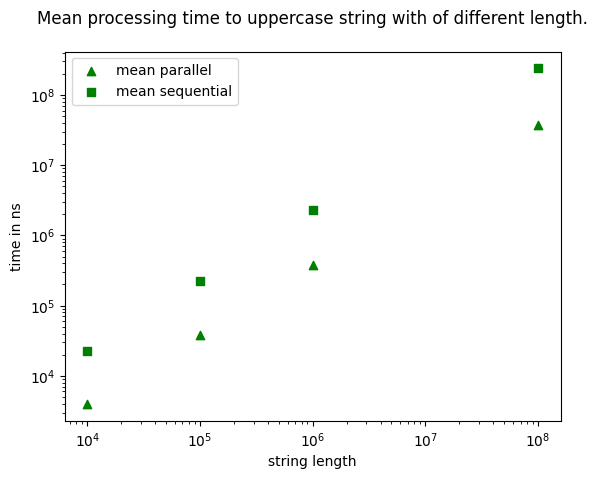
\includegraphics[width=0.7\textwidth]{images/complex_upper.png}
		\caption{Durchschnittliche Durchführungszeit von toUppercase() in Abhängigkeit von der Stringlänge.}
		\label{fig:mean_upper}
	\end{center}
\end{figure}

\begin{figure}[h]
	\begin{center}
		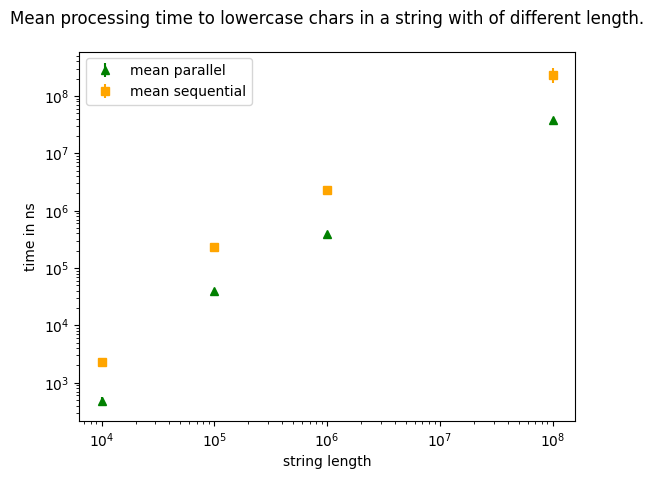
\includegraphics[width=0.7\textwidth]{images/complex_lower.png}
		\caption{Durchschnittliche Durchführungszeit von toLowercase() in Abhängigkeit von der Stringlänge.}
		\label{fig:mean_upper}
	\end{center}
\end{figure}

\begin{figure}[h]
	\begin{center}
		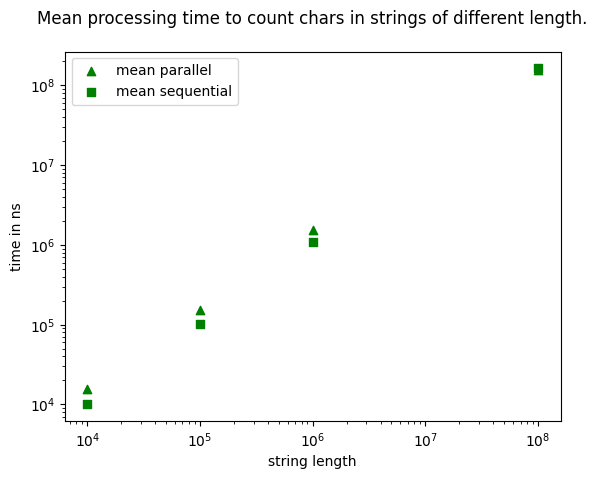
\includegraphics[width=0.7\textwidth]{images/complex_count.png}
		\caption{Durchschnittliche Durchführungszeit von countChar() in Abhängigkeit von der Stringlänge.}
		\label{fig:mean_upper}
	\end{center}
\end{figure}


\subsection{Ausführungszeiten}
\subsubsection{toUppercase}
In der Tabelle \ref{Tab:uppertab} sind die Zeitmessungen für die toUppercase() Funktionen zusammengefasst.
Es ist deutlich zu sehen, dass die se­quen­ti­elle Ausführung in für jede Stringlänge mehr Zeit benötigt als die Umsetzung mit SIMD.
\newline
\begin{tabular}{|c|r|l|r|l|}
	\hline
	\multicolumn{1}{|c|}{String Länge} & \multicolumn{2}{c|}{parallel in ns} & \multicolumn{2}{c|}{se­quen­tiell­ in ns} \\
	\cline{2-5}
	& Mittelwert & Standardabweichung  & Mittelwert & Standardabweichung \\
	\hline
	%\input{tabulars/lower_tab.txt} does some weird stuff and I was unable to figure out why
	10000 & 3941.83 & 99.05 & 22770.56 & 742.42 \\
	100000 & 37887.05 & 956.77 & 226738.36 & 2999.89 \\
	1000000 & 377705.08 & 5983.36 & 2266248.56 & 49165.20 \\
	100000000 & 37870118.15 & 251997.62 & 239285340.75 & 15524013.02 \\
	\hline
\end{tabular}
\label{Tab:uppertab}


\subsubsection{toLowercase}
In der Tabelle \ref{Tab:lowertab} sind die Zeitmessungen für die toLowercase() Funktionen zusammengefasst.
Es ist deutlich zu sehen, dass die sequentielle Ausführung in für jede Stringlänge mehr Zeit benötigt als die Umsetzung mit SIMD.
\newline
\begin{tabular}{|c|r|l|r|l|}
	\hline
	\multicolumn{1}{|c|}{String Länge} & \multicolumn{2}{c|}{parallel in ns} & \multicolumn{2}{c|}{sequentiell in ns} \\
	\cline{2-5}
	& Mittelwert & Standardabweichung  & Mittelwert & Standardabweichung \\
	\hline
	%\input{tabulars/upper_tab.txt} does some weird stuff and I was unable to figure out why
	10000 & 3911.31 & 53.24 & 22833.18 & 1071.49 \\
	100000 & 37892.37 & 1033.47 & 226494.29 & 2239.45 \\
	1000000 & 379459.13 & 7819.23 & 2267153.78 & 53847.50 \\
	100000000 & 37925051.64 & 281477.97 & 237236163.45 & 14932397.49 \\
	\hline
\end{tabular}
\label{Tab:lowertab}

\subsubsection{countChar}
In der Tabelle \ref{Tab:counttab} sind die Zeitmessungen für die countChar() Funktionen zusammengefasst.
Es ist zu sehen, dass die sequentielle Ausführung in für jede Stringlänge mehr Zeit benötigt als die Umsetzung mit SIMD. Hier ist der Unterschied allerdings nicht so deutlich wie bei den vorherigen Funktionen. Hier würde es sich lohnen nach einer effizienteren Lösung zu suchen als dem aktuellen Ansatz.

Desweiteren ist die Standardabweichung auffällig hoch für den sequentiellen Ansatz bei einer Stringlänge von 100 Millionen. Deutlicher zu sehen in Abb. \ref{fig:count_comp_100M}.
\newline
\begin{tabular}{|c|r|l|r|l|}
	\hline
	\multicolumn{1}{|c|}{String Länge} & \multicolumn{2}{c|}{parallel in ns} & \multicolumn{2}{c|}{sequentiell in ns} \\
	\cline{2-5}
	& Mittelwert & Standardabweichung  & Mittelwert & Standardabweichung \\
	\hline
	%\input{tabulars/count_tab.txt} does some weird stuff and I was unable to figure out why
	10000 & 2661.56 & 407.58 & 10033.59 & 370.35 \\
	100000 & 25458.25 & 518.46 & 102091.97 & 2537.17 \\
	1000000 & 254677.21 & 6522.01 & 1023648.08 & 13778.45 \\
	100000000 & 25652750.79 & 87472.48 & 147403368.22 & 58081046.77 \\

	\hline
\end{tabular}
\label{Tab:counttab}

\newpage
\subsection{Vergleich}
In den folgenden Abbildungen sind 100 Laufzeiten für das Verarbeiten eines Strings aufgezeigt. Dabei sind pro Funktion 4 Abbildungen für je 10.000, 100.000, 1.000.000 und 100.000.000 Zeichen in den Strings. Die Diagramme veranschaulichen den Vergleich zwischen dem sequentiellen und parallelen Ansatz unter Verwendung von SIMD.
\subsubsection{toUppercase}
Alle Diagramme zeigen deutlich, dass der parallele Ansatz schneller ist für alle Stringlängen.
\begin{figure}[h]
	\begin{center}
		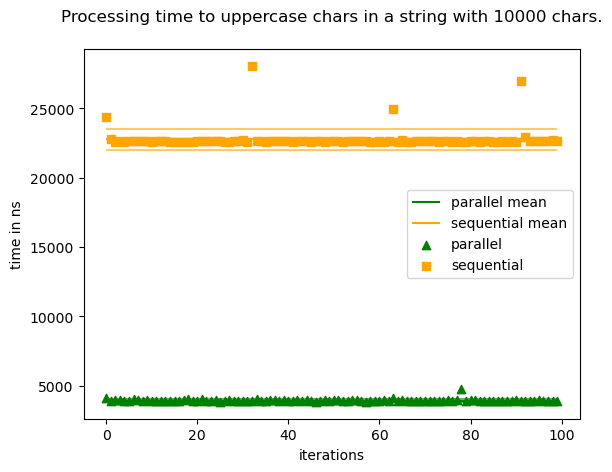
\includegraphics[width=0.65\textwidth]{images/comp_upper_10000.png}
		\caption{Durchführungszeiten von toUppercase für einen String mit 10.000 Zeichen.}
	\end{center}
\end{figure}
\begin{figure}[h]
\begin{center}
	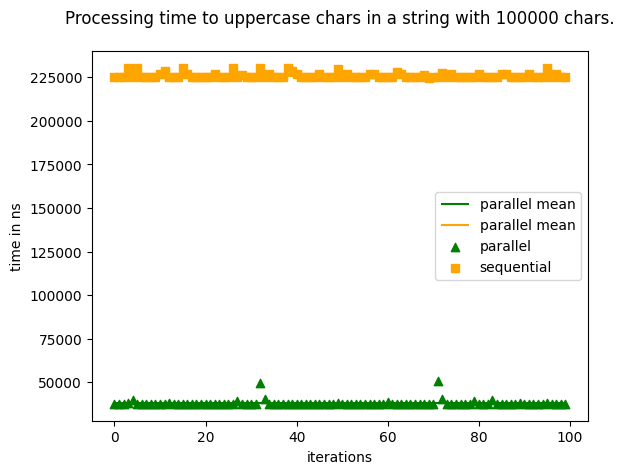
\includegraphics[width=0.65\textwidth]{images/comp_upper_100000.png}
	\caption{Durchführungszeiten von toUppercase für einen String mit 100.000 Zeichen.}
\end{center}
\end{figure}
\begin{figure}[h]
\begin{center}
	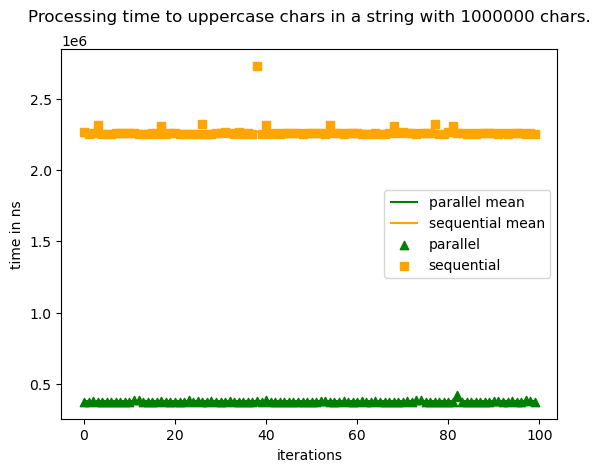
\includegraphics[width=0.65\textwidth]{images/comp_upper_1000000.png}
	\caption{Durchführungszeiten von toUppercase für einen String mit 1.000.000 Zeichen.}
\end{center}
\end{figure}
\begin{figure}[h]
\begin{center}
	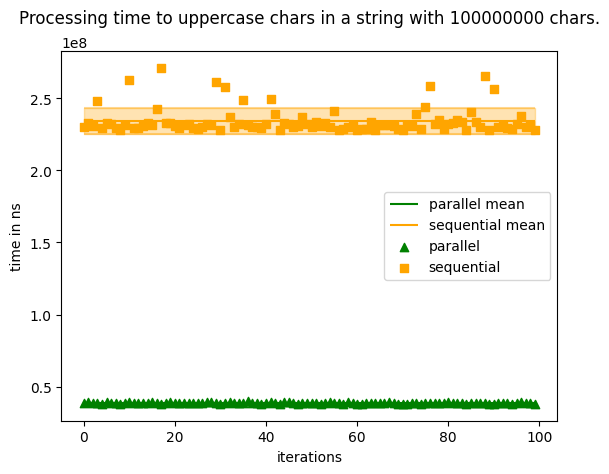
\includegraphics[width=0.65\textwidth]{images/comp_upper_100000000.png}
	\caption{Durchführungszeiten von toUppercase für einen String mit 100.000.000 Zeichen.}
\end{center}
\end{figure}

\clearpage
\subsubsection{toLowercase}

Alle Diagramme zeigen deutlich, dass der parallele Ansatz schneller ist für alle Stringlängen.
\begin{figure}[h]
	\begin{center}
		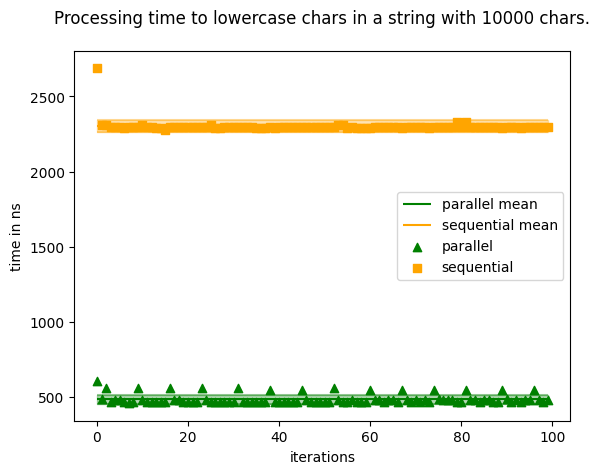
\includegraphics[width=0.65\textwidth]{images/comp_lower_10000.png}
		\caption{Durchführungszeiten von toLowercase für einen String mit 10.000 Zeichen.}
	\end{center}
\end{figure}
\begin{figure}[h]
	\begin{center}
		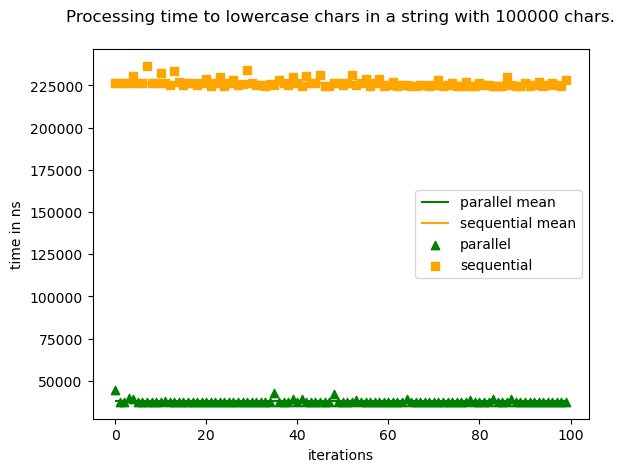
\includegraphics[width=0.65\textwidth]{images/comp_lower_100000.png}
		\caption{Durchführungszeiten von toLowercase für einen String mit 100.000 Zeichen.}
	\end{center}
\end{figure}
\begin{figure}[h]
	\begin{center}
		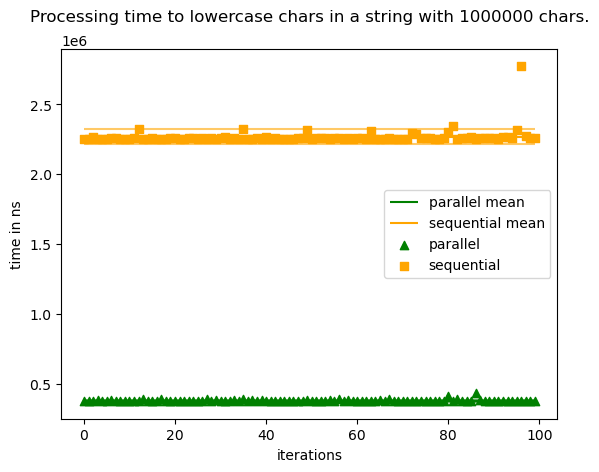
\includegraphics[width=0.65\textwidth]{images/comp_lower_1000000.png}
		\caption{Durchführungszeiten von toLowercase für einen String mit 1.000.000 Zeichen.}
	\end{center}
\end{figure}
\begin{figure}[h]
	\begin{center}
		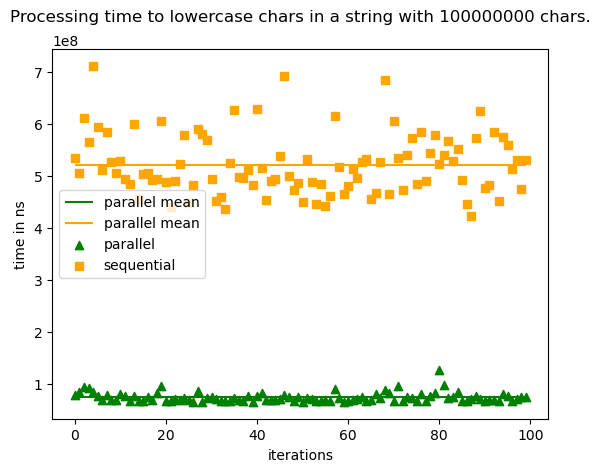
\includegraphics[width=0.65\textwidth]{images/comp_lower_100000000.png}
		\caption{Durchführungszeiten von toLowercase für einen String mit 100.000.000 Zeichen.}
	\end{center}
\end{figure}

\clearpage
\subsubsection{countChar}
Die folgenden Diagramme zeigen jeweils 100 Laufzeiten für einen String mit unterschiedlicher Länge. Gemessen wird die Laufzeit um einen gegebenen Buchstaben ('c') im String zu zählen.

Auch hier ist zu sehen, dass der parallele Ansatz deutlicher schneller ist. 

In Abb. \ref{fig:count_comp_100M} ist ein sehr merkwürdiges Verhalten für die sequentielle Lösung zu sehen. Für den gleichen String scheint die Funktion entweder extrem schnell oder langsam zu sein. Da es der gleiche String ist, kann der Grund nicht sein, dass die Anzahl der Vorkommen von 'c' eine derartigen Unterschied erzeugen. Der Unterschied tritt auch erst mit der hohen Stringlänge auf, allerdings nicht bei 'lowercase' und 'uppercase' also sollte das Problem auch nicht in bei Speichermangel etc. liegen.
Ich konnte das gleiche Verhalten bei meinem Laptop nicht beobachten und kann es auch nicht sicher erklären.

\begin{figure}[h]
	\begin{center}
		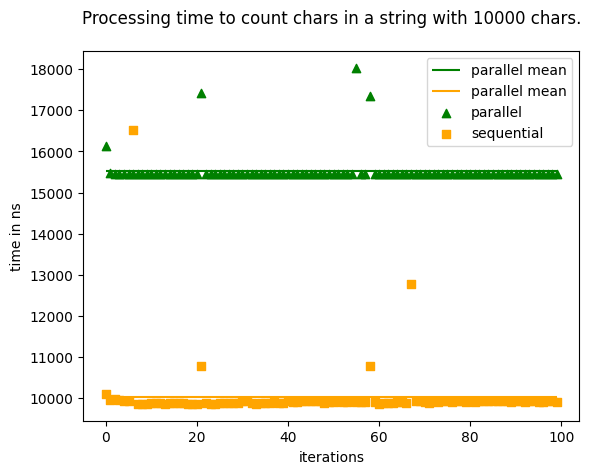
\includegraphics[width=0.55\textwidth]{images/comp_count_10000.png}
		\caption{Durchführungszeiten von countChars für einen String mit 10.000 Zeichen.}
	\end{center}
\end{figure}
\begin{figure}[h]
	\begin{center}
		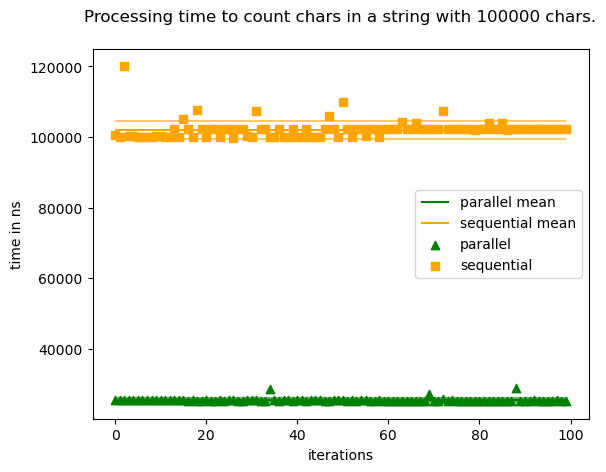
\includegraphics[width=0.55\textwidth]{images/comp_count_100000.png}
		\caption{Durchführungszeiten von countChars für einen String mit 100.000 Zeichen.}
	\end{center}
\end{figure}
\newpage
\begin{figure}[h]
	\begin{center}
		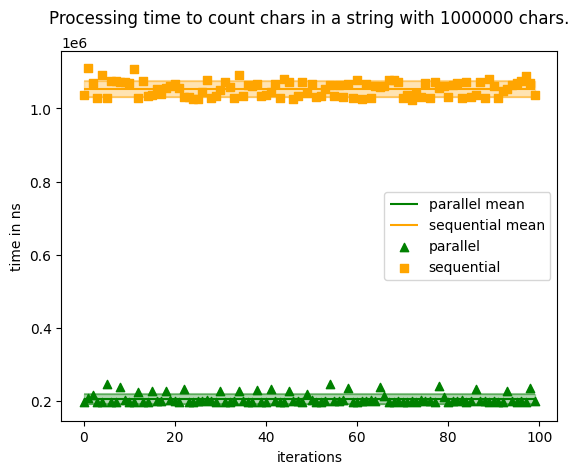
\includegraphics[width=0.55\textwidth]{images/comp_count_1000000.png}
		\caption{Durchführungszeiten von countChars für einen String mit 1.000.000 Zeichen.}		
	\end{center}
\end{figure}
\begin{figure}[h]
	\begin{center}
		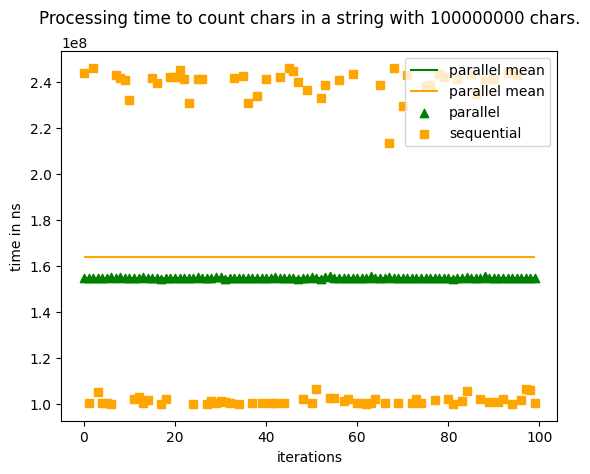
\includegraphics[width=0.55\textwidth]{images/comp_count_100000000.png}
		\caption{Durchführungszeiten von countChars für einen String mit 100.000.000 Zeichen.}
		\label{fig:count_comp_100M}
	\end{center}
\end{figure}

\newpage
\begin{thebibliography}{9}
	\bibitem{hakmem_count}
	Jeu George's Blog 'Parallel Counting'\newline \url{https://web.archive.org/web/20151229003112/http://blogs.msdn.com/b/jeuge/archive/2005/06/08/hakmem-bit-count.aspx}
	
	\bibitem{hpc_compendium}
	HPC Compendium, 'HPC Resources', 12.01.2024
	\url{https://doc.zih.tu-dresden.de/jobs_and_resources/hardware_overview/#romeo}
\end{thebibliography}

\end{document}